\documentclass[conference]{IEEEtran}
\usepackage[utf8]{inputenc}
\usepackage{graphicx}
\usepackage{epstopdf}
\usepackage{listings}
\usepackage{url}
\ifCLASSINFOpdf
  % \usepackage[pdftex]{graphicx}
  % declare the path(s) where your graphic files are
  % \graphicspath{{../pdf/}{../jpeg/}}
  % and their extensions so you won't have to specify these with
  % every instance of \includegraphics
  % \DeclareGraphicsExtensions{.pdf,.jpeg,.png}
\else
  % or other class option (dvipsone, dvipdf, if not using dvips). graphicx
  % will default to the driver specified in the system graphics.cfg if no
  % driver is specified.
  % \usepackage[dvips]{graphicx}
  % declare the path(s) where your graphic files are
  % \graphicspath{{../eps/}}
  % and their extensions so you won't have to specify these with
  % every instance of \includegraphics
  % \DeclareGraphicsExtensions{.eps}
\fi
\lstdefinelanguage{ViewsetDSL}{showstringspaces=false,
    breaklines=true,
    tabsize=2,
    basicstyle=\ttfamily\footnotesize,
    morekeywords={usecase,
      interaction,
      withviewset,
      input,
      event,
      list,
      viewset,
      end,
      create,
      cancel,
      delete,
      save,
      exit,
      open_phonebook,
      add_new,
      ManagePhonebook,
      ListOfPersons,
      Edit,
      MainMenu,
      AddNewPerson,
    },
    otherkeywords={>,:},
    sensitive=false,
}
\lstdefinelanguage{ViewsetDSLMeta}{showstringspaces=false,
    breaklines=true,
    tabsize=2,
    basicstyle=\ttfamily\footnotesize,
    morekeywords={Model,
      ModelElement,
      Include,
      ViewSet,
      InteractionElement,
      InputElement,
      EventElement,
      ListElement,
      Mapping,
      UseCase,
      Interaction,
      AbstractInteraction,
      NavigationRule,
      FillString,
      Punctuation,
    },
    sensitive=true,
}
\lstset{frame=single,boxpos=t}

\begin{document}

\title{A Textual Domain Specific Language for\\
User Interface Modelling}
\author{\IEEEauthorblockN{Mart Karu}
\IEEEauthorblockA{Department of Informatics, Tallinn University of Technology,\\
Raja 15, 12618 Tallinn, Estonia\\
karu@metal.ee}
}
\maketitle

\begin{abstract}
User interface development is one of the hardest parts of the software
application development. It could be made more efficient by introducing
model-driven development approaches and user interface modelling.  This paper
introduces a textual domain specific language and a corresponding meta-model
for describing user interaction using abstract UI patterns that can be
transformed into more platform specific UI patterns during application
generation. The language also follows use case description format and provides
possibilities to add free-form documenting context to the formal constructs
used in the language, making the models described in the language suitable both
for model driven engineering and requirements elicitation.
\end{abstract}

\IEEEpeerreviewmaketitle

\begin{figure*}
  \centering
    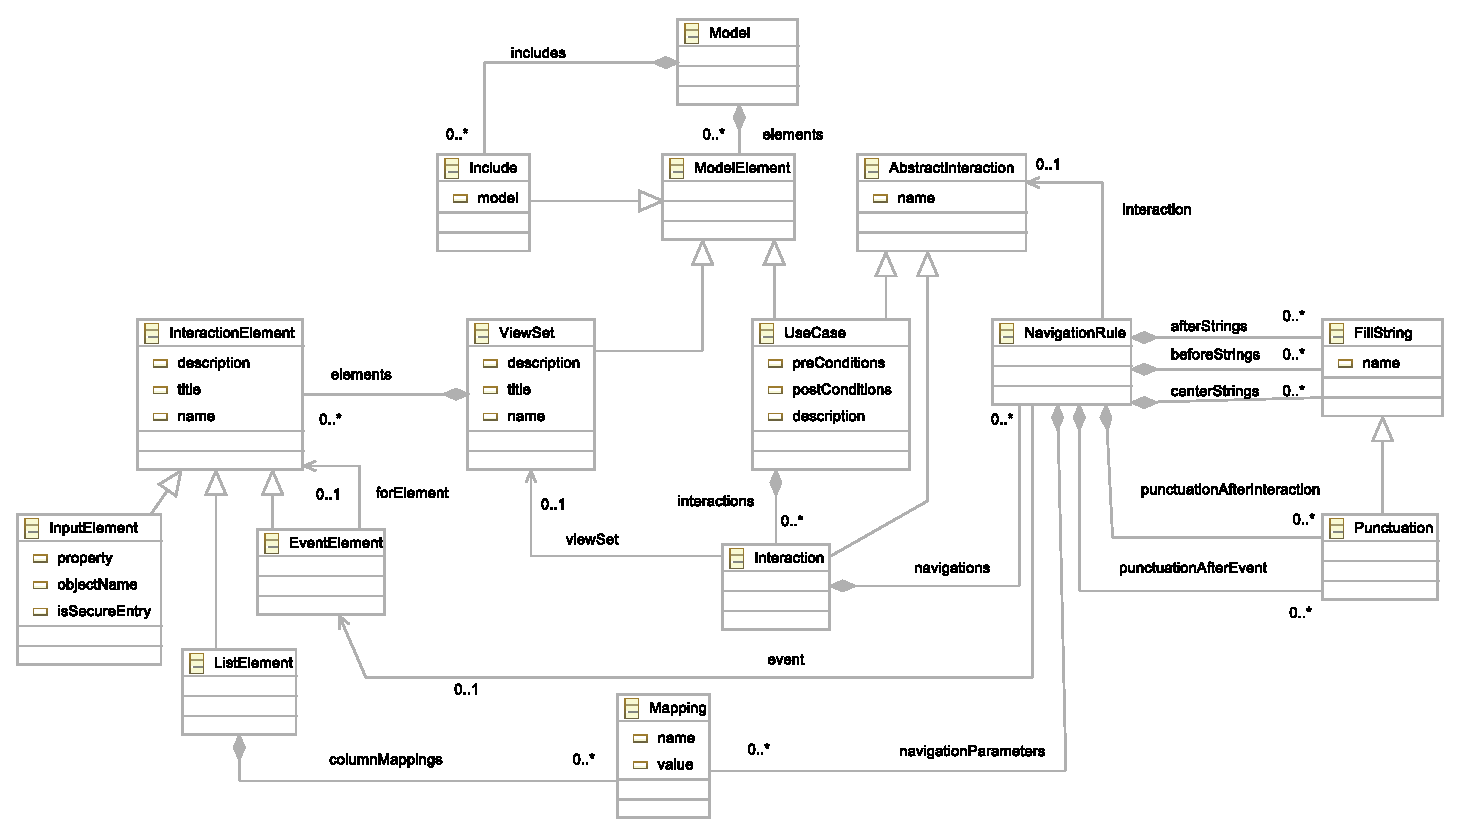
\includegraphics[width=1\textwidth]{viewsetdsl.eps}
      \caption{Meta-model supported by the language}
      \label{fig:metamodel}
\end{figure*}

\section{Introduction}
User interface (UI) development is one of the hardest parts of a software
development, especially in a world where the success of a software application
can be attributed to the quality and consistency of its UI\@. Targeting UI
development with model driven development (MDD) methods can:

\begin{itemize}
  \item reduce the effort needed to implement and maintain reoccurring UI
    patterns in general purpose languages, by abstracting out the patterns to
    the meta-model and to the corresponding modeling language.
  \item raise the quality and consistency of the application UI, by applying
    code generation techniques that will always produce similar implementations
    of the patterns across the target application.
\end{itemize}

The goal of this paper is to introduce an additional language and a
corresponding meta-model to the existing user interface modelling languages and
meta-models, that could raise the quality of the viewpoint taken on a model and
on the general domain of UI modelling and model driven UI development.

This paper is organised into six sections.  Section 2 explains the other
related works in this field and motivation behind the work.  Section 3
describes the proposed language and the concept space the language covers.
Section 4 will give an exemplifying overview of the language usage.  Section 5
discusses the results of the work and the final section will conclude the work.

\section{Related Work and Motivations}

Current modelling languages used in MDD-specific UI modelling can be divided
into three categories based on the modelling approach:

\begin{itemize}
  \item UML-based languages and UML Profiles
  \item Graphical Domain Specific modelling languages
  \item Textual Domain Specific modelling languages
\end{itemize}

The UML-based approaches rely on using standard UML concepts like class and
interaction diagrams \cite{Silva00userinterface} or specific UML profiles
\cite{KochKraus02expressivepower} that further restrict the generic UML
language by applying domain specific constraints. While the approaches do
manage to capture the most essential parts of the UI and there is mature tool
support available, the complexity of the UML meta-models and the inflexibility
of the standard diagram formats to be tailored to match the domain make them
not the most optimal choice for the MDD in general
\cite{KellyTolvanen08DomainSpecific}.

Non-UML based graphical languages have the freedom to use the most suitable
language representation for UI modelling and there are several works
\cite{Trtteberg01modelbased,Ceri00webmodeling,Goderis04adeclarative} that
utilise graphical modelling languages or visual toolsets. While the graphical
languages are prevailing approaches to the UI modelling and there are clear
benefits of using graphical languages, there are also disadvantages when
compared to textual languages \cite{GronnigerKrahn07TextbasedModeling}.

On the existing textual languages side, there are domain specific languages
(DSL) for developing web-based user interfaces like WebDSL \cite{Visser_2008}
attempts to describe the UI domain using functional languages
\cite{Plasmeijer2009}. Also the UsiXML approach \cite{Limbourg04} can be
considered to be based on the textual XML language, although in practice the
XML is being generated from the graphical modelling tool front-ends
\cite{Vanderdonckt05}.

Concept-space wise, many model driven approaches employ meta-models that
include concepts that are based directly on a specific technical target
platform or UI style. For example, in the WebDSL approach the UI aspects are
describe by using idioms and UI elements widely known in the web-based UIs.
There are works that express the importance of using more abstract ways of
marking UI concepts and using intelligent transformations
\cite{Borchers2000,AhmedAshraf2007} or abstract UI modelling in general
\cite{Limbourg04}.

Based on the previous works and the benefits
\cite{KellyTolvanen08DomainSpecific} of MDD, it would be reasonable to
construct a domain specific textual language that would satisfy the following
goals:

\begin{itemize}
  \item The language needs to present a model as a first class artefact for
    capturing requirements of all of the aspects of the user interaction.
  \item The model described by the language needs to be formal enough to be
    used in user interface generation using MDD approaches.
  \item The language (and the meta-model) should have extension points for
    integrating the target model with models that represent other software
    application domains
  \item The language should present the user interaction patterns in the
    abstract form, to facilitate independence from the user interface
    technology and the interaction paradigm.
  \item The language should be textual because of the many practical benefits
    of the textual languages, like efficient creation and maintenance,
    efficient usage of visual space, language integration possibilities, fast
    formatting, version control and mature tool support
    \cite{GronnigerKrahn07TextbasedModeling}.
\end{itemize}

\section{Overview of the Language}

The UI description language and the corresponding meta-model described in this
paper operates with the concepts that have a variable nature in the UI domain
space. The language and the meta-model consist of two distinct parts. The first
part describes the aspects and the granularity of the interaction elements
provided to the system user during each interaction step. The second part of
the language describes all of the possible interactions provided by the UI.

The meta-model allows inclusion of other UI model instances by using special
language construct ‘include’ and a corresponding meta-model element Include.

\subsection{View-sets and Interaction Elements}

The limitations of human perception require the user interfaces to quantify the
amount of information and interaction possibilities that are expressed to the
user interface user.  The first goal of the UI description language is to
capture the sets or partitions of the user interface elements that are made
available to the system user during each interaction step.

The interaction elements that are referenced in the language are expressed as
abstract patterns that will be transformed into more precise patterns during
model transformations towards executable software application.

The following list of the most basic abstract patterns is incorporated into the
language as an example for this paper:

\begin{itemize}
  \item data entry - an ability to enter simple stream of data to the system.
  \item secure data entry - an ability to securely enter data to the system.
  \item list of selectable items - a list of items where one of the items can
    be selected and the corresponding event to be generated.
  \item event firing - an ability to produce events to be processed by the
    system.
\end{itemize}

When an interaction element is placed into the model, the abstract UI pattern
it references will be instantiated with the provided parameters that will
configure the variable parts of the pattern.  For example, adding the keyword
"secure" to the regular input element will denote that the inputs presentations
in lower abstraction levels must follow a platform-specific pattern that would
guarantee secure entry while inputting the data.

The interaction elements are grouped into viewsets by using the keyword
“viewset”.  The viewset definition and each element can be named and can also
have two descriptive strings placed after the definition.  The first string
denotes a title of the element or the viewset and the second one gives a
description of the object.

Both strings are useful during transformations - the title string can show the
purpose of the element in the graphical UIs and the description string can be
transformed to context-specific help messages accompanying the element.

\subsection{Navigation and Interaction}

To retain the most common appearance of the requirement artefact, the starting
point in design of the interaction description part of the UI language has been
the classic use case description format \cite{Cockburn10template}.  The use
case scenarios are presented as separated interactions with a reference to a
viewset that is being used to carry out the interaction.  The
\textit{Interactions} are contained inside the \textit{UseCase} container to
group logically related interactions.  Each \textit{Interaction} contains:

\begin{itemize}
  \item optional freeform textual description or documentation of the
    interaction
  \item markings inside the freeform text to connect events described in the
    viewsets and the next interactions to be initiated after the events.
\end{itemize}

The references to the viewset's events are prefixed with the character ":" and
references to following interactions or usecases with the character
"\textgreater".  Together those markings form an event-to-reaction navigation
pair that can be used to construct the interaction graph.  This syntax enables
to describe the navigational graph state-machine in textual form and also
provides documentation context to the use case description.  If
\textit{Interaction} names and use case names are chosen appropriately, a
clear, readable and yet formal enough textual description of the user
interaction can be specified.

In the meta-model, both \textit{UseCase} and \textit{NavigationRule} elements
are defined as special cases of \textit{AbstractInteraction} element. It allows
the \textit{NavigationRule} elements (defined by the event-to-reaction syntax)
to reference either other interactions or use cases. This allows the navigation
targets to be either large scale use cases or interactions inside a specific
use case.  \textit{NavigationRules} are defined in the \textit{Interaction} and
the \textit{Interaction} elements are placed in the \textit{UseCase} elements.
The \textit{NavigationRule} element also references the \textit{EventElement}
that initiates a navigational change in the UI.

To be usable as a general requirement specification artefact, the other
elements of the use case description format can be added to the language.
Although only the simplest way of marking the use case interactions is
presented in this paper, the other conditions and markings available in use
case descriptions could be evolved to be more formal and more tightly
integrated with other domain areas, like role-based security or other business
domain areas.

\subsection{Integration with Other Domains}

The UI aspects are rarely isolated from the other aspect models that define a
software application. The integration with the core business domain models is
implemented by referencing the name of the business domain service to be
invoked as a response to the event. The returned data of the service can be
stored in the named slots and can be used in the viewsets that are displayed
after the event. The named slots are stored in the model as the meta-model
\textit{Mapping} elements. The parameters given to the business service can be
resolved during source code generation by passing the interaction context (the
interaction and the corresponding viewset) object as a parameter.

\subsection{Formal Definition of the Language}

\begin{figure}
  \begin{lstlisting}[language=ViewsetDSLMeta]
  Model:
    (includes += Include)*
    (elements += ModelElement)*;
  ModelElement:
    ViewSet | UseCase | Include;
  Include:
    "include" model = URI;
  ViewSet:
    "viewset" name = ID (title = STRING)?
    (description = STRING)?
    (elements += InteractionElement)* "end";
  InteractionElement:
    InputElement | EventElement | ListElement;
  InputElement:
    (isSecureEntry ?= "secure")?
    "input" name = ID (title = STRING)?
    (description = STRING)?
    ("(" objectName = ID
      ("." property = ID )? ")")?;
  EventElement:
    "event" (forElement = [InteractionElement] ".")?
    name = ID
    (title = STRING)? (description = STRING)?;
  ListElement:
    "list" name = ID (title = STRING)?
    (description = STRING)?
    "(" (columnMappings += Mapping)* ")";
  Mapping:
    name = ID ":" value = ID;
  UseCase:
    "usecase" name = ID (description = STRING)?
      (interactions += Interaction)*
     "end";
  Interaction:
    "interaction" name = ID 
    ("withviewset" viewSet = [ViewSet])?
    (navigations += NavigationRule)* "end";
  AbstractInteraction: UseCase | Interaction;
  NavigationRule:
    (beforeStrings += FillString)*
    ":" event = [EventElement]
    ( "(" navigationParameters += Mapping ")")?
    (punctuationAfterEvent += Punctuation)*
    (centerStrings += FillString)*
    ">" interaction = [AbstractInteraction]
    (punctuationAfterInteraction += Punctuation)*
    (afterStrings += FillString)*;
  FillString:
    name = ID (Punctuation)*;
  Punctuation:
    "." | "," | "!" | "\-";
  \end{lstlisting}
  \caption{Language grammar definition}
  \label{fig:grammar}
\end{figure}


Based on the examples and features described above, a grammar (displayed in
figure \ref{fig:grammar}) and a corresponding meta-model (displayed in figure
\ref{fig:metamodel}) can be expressed to support the language. The grammar
definition is expressed using the grammar definition DSL of the Xtext
programming language framework \cite{EfftingeVolter06}.  The metamodel is
expressed as an instance of the Ecore meta-meta-model \cite{EclipseModeling10}.

\subsection{Integrating with Model Driven methodologies}

The abstraction level of the language and of the corresponding meta-model
enables platform independence from the user interface technology and
interaction paradigm. The model can be transformed into both graphical UIs and
conversational UIs, like voice based or command-line interfaces. Since the
communicational UIs are based on few simple interface patterns like detecting
or parsing speech or text and responding with speech or text, the abstract
patterns defined in the UI model can be implemented by combining the simple UI
patterns supported by the conversational UI platform.

The model described by the language can be used in custom-made transformations
or can be applied to other user interface transformation approaches. To use the
model with other approaches, a model-to-model transformation is needed to
transform the model concepts into the concept space of the target meta-model.

\begin{figure}
  \centering
    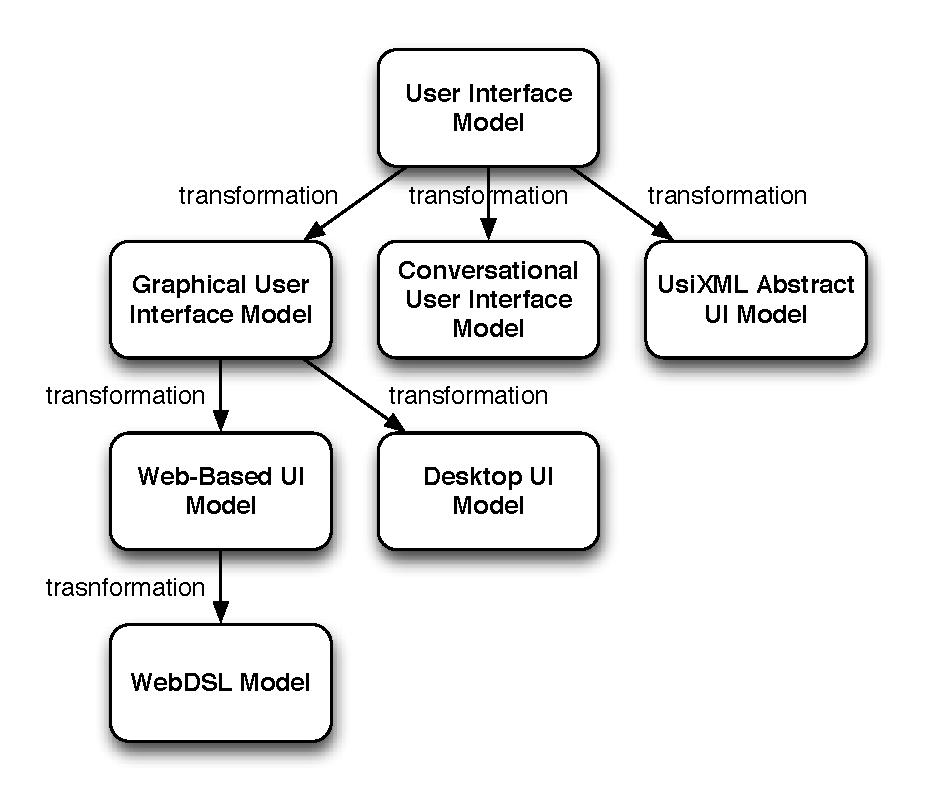
\includegraphics[width=0.5\textwidth]{transformations.eps}
      \caption{Model transformation paths}
      \label{fig:transformation_paths}
\end{figure}

Since the model relies on abstract patterns, the abstract patterns must be
transformed into platform specific patterns during model transformations. The
figure \ref{fig:transformation_paths} shows some possible transformation paths
from the UI model to more reified platform specific models.

\section{Example Usage}

\begin{figure}
  \begin{lstlisting}[language=ViewsetDSL]
  usecase MainMenu "Main menu"

    interaction ShowPhoneBook withviewset MainMenu
      User can :open_phonebook(people:getpersons)
      and the >ManagePhonebook section will
      be showed.
    end

    usecase ManagePhonebook "Phonebook Manager"

      interaction ListOfPersons withviewset PhoneBook
        User needs to :select a person from the
        list of persons to >Edit the person data.
        If user wants to :add_new person then the
        >AddNewPerson form must be filled.  User
        can :exit the phonebook and to return
        to the >MainMenu.
      end

      interaction Edit withviewset EditPhoneBookEntry 
        User modifies the Person data and
        initiates :save(people:getpersons) to store
        the changes.  The system responds
        with >ListOfPersons.  If the user wants
        to :cancel(people:getpersons) editing, no
        changes are stored and the user will be
        directed to >ListOfPersons.  To remove a
        person user must :delete(people:getpersons)
        and after that the >ListOfPersons will
        be shown.
      end

      interaction AddNewPerson
          withviewset EditPhoneBookEntry
        To :create(people:getpersons) a new person,
        user enters and saves person data and the
        >ListOfPersons will be shown.  If the user
        wishes to :cancel(people:getpersons) new
        person creation the >ListOfPersons
        will be displayed.
      end

    end

    viewset MainMenu
      event open_phonebook "Open phonebook"
    end

    viewset PhoneBook
      list people "People in the phonebook:"
         (Name:name Number:number)
      event people.select "Edit"
      event add_new "Add new person"
      event exit "Exit"
    end

    viewset EditPhoneBookEntry "Person data entry"
      input name "Name" "Name of the person"
      input number "Phone number"
        "Phone number of the person"
      event save "Save"
      event create "Create"
      event delete "Delete"
      event cancel "Cancel"
    end
  end
  \end{lstlisting}
  \caption{Example usage of the UI DSL language}
  \label{fig:example_usage}
\end{figure}

One of the most widely used large scale UI patterns is a simple resource
management pattern that includes showing a list of items of interest and means
to edit, remove and delete the items. The example displayed in the figure
\ref{fig:example_usage} shows a implementation of the pattern in the form of a
basic phonebook application. The example displays:

\begin{itemize}
  \item Two use cases (\textit{MainMenu} and \textit{ManagePhonebook}) that
    contain interaction descriptions.
  \item Descriptions of three viewsets (\textit{MainMenu}, \textit{PhoneBook}
    and \textit{EditPhoneBookEntry}) and the interaction patterns (inputs,
    events) used in the viewset.
\end{itemize}

The textual descriptions of the interactions contain event-to-reaction pairs.
For example, the :open\_phonebook event initiates a business service
getpersons and stores the result in the slot named people.

\begin{figure}
  \centering
    \includegraphics[width=0.5\textwidth]{webexample.png}
      \caption{Web-based application generated from the example model.}
      \label{fig:web_based_example}
\end{figure}

Figure \ref{fig:web_based_example} displays a fully functional web-based
application UI that was transformed from the model described in the example.

\section{Disussion}

The language and the corresponding meta-model are the results of the iterative
prototyping work using the Xtext language development framework
\cite{EfftingeVolter06}. The prototyping work also included a development of
model-to-model and model-to-code transformation rules that were used to
generate working implementations of the UIs on different technological and UI
platforms. The target implementations used in the prototype were:

\begin{itemize}
  \item Graphical web-based UI implemented in the Ruby language \cite{Ruby10}
    and on the Ruby on Rails framework \cite{Rails10}.
  \item Graphical desktop-based UI implemented on the Java Swing framework
    \cite{JavaxSwing10}.
  \item Text-based conversational UI implemented in the Python language
    \cite{Python10}.
  \item Voice-based conversational UI implemented in the C\# language
    \cite{Csharp10} using the Microsoft Speech voice recognition and synthesis
    API \cite{MsSpeech10}.
\end{itemize}

The generated target implementations were used as a feedback for verifying
the usability and suitability of the language and the meta-model. It also
helped to unify the concepts of target platforms as the abstract concepts in
the meta-model.

The iterative process of improving the work results has proved the meta-model
and the language to be sufficient enough for the narrow context of supporting
the code generation of the selected target platform UIs. More thorough
assessment of the quality and usability of the language must be measured, based
on either of the comparison of other similar languages or the fundamental
principles and best practices of language design.

Based on the principles described in \cite{PaigeOstroffBrooke2000}, the
language and the meta-model described in this paper can be evaluated using the
following quality aspects:

\begin{itemize}
  \item Simplicity: The proposed UI language and the meta-model provide
    narrowly focused and minimal concepts for describing UIs. Accidental
    complexity by adding confusing language elements has been avoided.
  \item Uniqueness: The meta-model consists of unique elements that do not
    overlap conceptually.
  \item Consistency: The proposed language lets to connect the meta-model
    concept instances and the instantiated models contain the formal
    description of the UIs. All the language elements support the initial
    language development goals.
  \item Seamlessness: The abstractions provided by the language can be used
    repeatedly throughout the development process and the resulting models
    can be used to generate working software implementations.
  \item Reversibility: Reverse-engineering the generated models or the source
    code back to the UI models is orthogonal to the language and meta-model
    described in this paper. Any reverse-engineering tool capable of detecting
    the required abstractions could output the collected knowledge as a textual
    UI model, using the proposed textual language.
  \item Scalability: The language can be used to describe both large and small
    systems, by separating the model descriptions into different text files.
  \item Supportability: The proposed language can be used both as the
    requirement artefact for human use and as a model for generating UI
    implementations.
  \item Reliability: The language facilitates pattern-based software
    generation, that will always produce similar (and tested) source code
    footprints for a specific pattern or a model concept.
  \item Space economy: Using the language without textual interaction
    description contexts could result in very concise textual representations.
    As the amount of the textual documentation included in the descriptions
    increases, the space needed to visualise the model also increases.
\end{itemize}

\section{Conclusion}

A textual domain specific language has been described in this paper that can be
used to define aspects of human-computer interaction. The resulting models and
their presentations could be used as generic artefacts for documenting software
requirements and also as formal models for UI generation. The concept space of
UI aspects used in the meta-model consist of the abstract UI patterns that can
be instantiated and configured in the UI models. The described models can be
used as inputs to various MDD scenarios and approaches that transform the
abstract patterns into more platform specific UI patterns in intermediate
models and later in the process into working UI implementations.

The example UI patterns in this paper cover only the most basic UI patterns and
domain integration possibilities. Also having a language defined based on the
use case format is just one possibility to expose the UI interaction model in a
domain specific language. The goals for the further work are the following:

\begin{itemize}
  \item Improving the language to support more complex integration scenarios by
    providing more integration extension points to the language.
  \item Mapping patterns and pattern transformations on various platforms so
    that more abstract patterns could be expressed in the language
  \item Provide a formalisation approach of similar text-based state-machine
    descriptions in agile user stories and scenarios, especially in the test
    automation tools that support Behaviour Driven Development \cite{Astels05}.
  \item Provide more through language quality evaluation based on the good
    modelling language principles and evaluation approaches.
  \item Compare the proposed language with other languages expressing similar
    concepts.
  \item Test the language and the meta-model in real-life development
    scenarios.
\end{itemize}

\section*{Acknowledgment}

This research was supported by the Estonian Doctoral School in Information and
Communication Technology

\bibliographystyle{ieeetr}
\bibliography{mddofui}

\end{document}


